\chapter{Methodology}
    \label{chap:methodology}

Chapter \ref{chap:methodology} details the methods relevant for this research. First, \ref{sec:method_haabsa} describes the baseline model HAABSA++ we aim to explain. Although a detailed explanation of the model is given in \cite{Trusca}, we will provide a basic explanation needed to understand the fundamentals of our research. Next, the working of the interpretation methods used to explain the HAABSA++ model will be detailed in \ref{sec:method_interpretation}. 

\section{HAABSA++}
    \label{sec:method_haabsa}
HAABSA++, which stands for Hybrid Approach to Aspect Based Sentiment Analysis, is a hybrid model designed to solve aspect based sentiment classification problems using a combination of an ontology and a deep learning model. The model first attempts to classify the sentiment towards a target using an ontology. When the ontology proves inconclusive, the model switches over to a deep learning model called LCR-Rot-hop++ \cite{Trusca}.

\subsection{Ontology}
    \label{sec:method_ontology}
The ontology is designed to find the possible sentiment expression of a word depending on the aspect. For instance, the word \textit{`small'} implies a positive sentiment in the context of \textit{`price'}, but a negative sentiment in the context of \textit{`portions'}. The model uses the NLTK platform to tokenize the text; each word is lemmatized based on the part-of-speech tagging using the WordNet lexical database within the NLTK platform. The ontology is manually constructed by \cite{Schouten} using the \textit{OntoClean} method \cite{Guarino}. Although \cite{Schouten} originally uses a support vector machine (SVM) model as backup method, a revised backup method by \cite{Wallaart} and then further improved by \cite{Trusca} proved to result in higher performance, leading to the final LCR-Rot-hop++ model. 

\subsection{LCR-Rot-hop++}
    \label{sec:method_lcrrothoppp}
LCR-Rot-hop++ utilizes BERT word embeddings to generate contextual word representations, as described by \cite{Devlin}. BERT allows for word embeddings that capture the semantic context of the words by averaging token vectors, position embeddings, and segment embeddings. In LCR-Rot-hop++ the BERT tokenization designed by the original authors of \cite{Devlin} is used to tokenize the text data. Afterwards the uncased base version of BERT containing 768 dimensions is used to generate word embeddings for our data.

LCR-Rot-hop++ then divides the sentence into three parts: left, center, and right. The target word(s) in the sentence are assigned as the center, while the remaining parts of the sentence are assigned towards the left or right part, depending on where they stand in relation to the target word. Looking at the previous example of Figure \ref{fig:review_snippet}, one recognizes two different target words in the sentence. When the target is defined as \textit{``service"}, then the left part consists of \textit{``Everything is always cooked to perfection, the"} and the right part of \textit{"is excellent, the decor cool and understated."}. If the sentence starts or ends with the target word, the left or right part will remain blank.

Each of the three parts are translated to their embedding representation defined by BERT. The left, center, and right part are then fed into a bidirectional Long Short-Term Memory (bi-LSTM) network as described in \cite{Cambria}, which produces three hidden state vectors. Bi-LSTMs combines two LSTMs, processing the text input in both a forward and backward order, to avoid bias towards words near the end of its sequence. The three hidden state vectors are then fed into a repeated two-step rotatory attention mechanism, rotating over a Target2Context and Context2Target mechanism for the left and right part sequentially, until the desired number of iterations has been reached.

To compute the Target2Context vector, an average pooling layer first produces a vector representation of the target phrase. Second, an attention mechanism assigns attention scores to the context, which are then normalized through a softmax function. The final context vector is computed by using a weighted combination of the hidden states.
The obtained context representation vector is used to adjust the target vector representation with a similar attention mechanism. Again, the computed attention scores are normalized through a softmax function and using a weighted combination of the hidden states the final target vector is obtained.
The four obtained vectors (target and context for both left and right sequences) are combined to calculate attention scores on the sentence level, scaling the context and target vectors one last time.
The second iteration uses the final obtained target vectors to replace the pooling layer in the first step, to reiterate the complete process for a total of three times.
Finally, the resulting vectors are concatenated to obtain the final sentence representation, which is fed into a Multi-Layer Perceptron (MLP) to compute the sentiment prediction vector, obtaining a sentiment prediction using a final softmax layer.


\section{Interpretation Methods}
    \label{sec:method_interpretation}
As the improved performance of the backup method has lead to an increase in complexity, a need has arisen to explain the model to better derive insights from the model predictions. This research utilizes SHAP to understand the features that contribute to the model predictions. 

\subsection{Shapley values}
    \label{sec:method_shapley}
Shapley values are a concept originally developed in cooperative game theory \cite{Shapley}, and have become more prominent in the field of machine learning since the introduction of SHAP \cite{Lundberg}. The aim is to calculate the exact contribution of each player, so that the value of each player can be distributed fairly. This concept has been adapted to the field of machine learning by interchanging players with features, so that the most important features in a machine learning model can be identified. The Shapley value evaluates all possible combinations of features in different coalitions, and calculates the output value of each coalition, which is then used to calculate the marginal contribution of each feature.

First we define the original sentence as the text including the context phrase and target phrase $\{W,\, T\} \in X$ in the sentence, where $W$ is the combination of all context words and $T$ the target phrase. Suppose we have a sentence with $N$ context words, then $W$ is the set of all context words $w_n$: $W=[w_1, w_2, \ldots, w_{N-1}, w_N]$. The nature of the LCR-Rot-hop++ model does not allow for target $T$ to be removed, because it uses the context words to predict the sentiment on $T$. Hence, the features for the SHAP model consist of the context words $w_n$ and the amount of features is equal to $N$. Each subset S includes a number of features $k$ between $[0,\;N]$ (i.e. varying between $\varnothing$ and the original sentence $W$). The amount of total possible subsets S is $2^N$. The power set of W is defined as all possible subsets S of W:

$$
P(W)= \{S \,|\, S \subseteq W\}
$$

Using an example of a sentence with $N = 4$ context words defined as $W=[w_1, w_2, w_3, w_4]$, table \ref{tab:shapley_subsets} shows all subsets in $P(W) \,|\, S \subseteq W$. The sentiment class probability of each subset is calculated by using the LCR-Rot-hop++ model described in \ref{sec:method_lcrrothoppp}. For every subset S we can obtain three different $p$-values: $[p_1,\; p_0,\; p_{-1}]$ for positive, neutral, and negative sentiment respectively. Depending on which $p$-value we use, we can calculate the Shapley value $\Phi_n$ of a word for that specific sentiment.

\begin{table}[h]
\caption{Example of the power set $P(W) \,|\, S \subseteq W,\, N=4$}
\centering
\begin{tabular}{c c c c c c}
\cmidrule(lr){2-6}
k: & 0 & 1 & 2 & 3 & 4\\ 
\cmidrule(lr){2-2} \cmidrule(lr){3-3} \cmidrule(lr){4-4} \cmidrule(lr){5-5} \cmidrule(lr){6-6}
&$[\varnothing]$ &   $[w_1]$ &   $[w_1,\; w_2]$ &    $[w_1,\; w_2,\; w_3]$   &   $[w_1,\; w_2,\; w_3,\; w_4]$    \\
&                &   $[w_2]$ &   $[w_1,\; w_3]$ &    $[w_1,\; w_2,\; w_4]$   &                                   \\
&                &   $[w_3]$ &   $[w_1,\; w_4]$ &    $[w_1,\; w_3,\; w_4]$   &                                   \\
&                &   $[w_4]$ &   $[w_2,\; w_3]$ &    $[w_2,\; w_3,\; w_4]$   &                                   \\
&                &           &   $[w_2,\; w_4]$ &                            &                                   \\
&                &           &   $[w_3,\; w_4]$ &                            &                                   \\ 
\bottomrule
\end{tabular}
\label{tab:shapley_subsets}
\end{table}

To calculate the Shapley value $\Phi_n$ of word $w_n$, formula \ref{formula: Shapley} is used. Here, $p(S)$ is defined as the $p$-value of subset S. Within the summation formula \ref{formula: Shapley}, this accounts for all subsets $S$ that do not contain $w_n$, as is denoted by $S \subseteq N \setminus \{w_n\}$. $p(S \cup \{w_n\})$ equals to the $p$-value of the subset where $w_n$ is added. Specifically, we calculate the difference between all subsets including $w_n$ and all subsets excluding $w_n$, to find the marginal $p$-value of adding $w_n$ to each subset. Then, the marginal value of the subset is divided by $\binom{N-1}{k(S)}$ before summed together. Last, the total sum is divided once more by N to obtain $\Phi_n$, which is the average marginal $p$-value of $w_n$.

\begin{equation}
    %\begin{aligned}
\label{formula: Shapley}
\Phi_{w_n} = \frac{1}{N} \sum_{S \subseteq N \setminus \{w_n\}} \frac{(p(S \cup \{w_n\}) - p(S))}{\binom{N-1}{k(S)}}
    %\end{aligned}
\end{equation} 

For instance, if we want to calculate the Shapley value of $w_1$, we calculate the marginal $p$-value of adding $w_1$ to each subset $S$ that does not contain $w_1$. Table \ref{tab:shapley_w1} shows each subset $S \setminus \{w\}$ and the subset after $\{w_1\}$ is added. The marginal $p$-value is the difference in $p$-value for each subset and its counterpart. The marginal $p$-value is divided by $\binom{N-1}{k}$ to obtain the average marginal value for each $k=i$. The total sum is divided once more by $N$ to obtain the total average marginal $p$-value for $w_1$. This process is done for all three sentiment classes, leading to three average marginal $p$-values of $w_1$.

\begin{table}[h]
\caption{All subsets $S \subseteq W \setminus \{w_1\} \,|\,N=4$ and union $\{w_1\}$}
\centering
\begin{tabular}{c c c c}
$k$ & $\binom{N-1}{k}$ &$S \cup \{w_n\}$ & $S \setminus \{w_1\}$ \\ 
\cmidrule(lr){1-2} \cmidrule(lr){3-3} \cmidrule(lr){4-4} 
0   &   1   &   $[w_1]$                         &   $\varnothing$           \\
1   &   3   &   $[w_1,\; w_2]$                  &   $[w_2]$                 \\
1   &   3   &   $[w_1,\; w_3]$                  &   $[w_3]$                 \\
1   &   3   &   $[w_1,\; w_4]$                  &   $[w_4]$                 \\
2   &   3   &   $[w_1,\; w_2,\; w_3]$           &   $[w_2,\; w_3]$          \\
2   &   3   &   $[w_1,\; w_2,\; w_4]$           &   $[w_2,\; w_4]$          \\
2   &   3   &   $[w_1,\; w_3,\; w_4]$           &   $[w_3,\; w_4]$          \\
3   &   1   &   $[w_1,\; w_2,\; w_3,\; w_4]$    &   $[w_2,\; w_3,\; w_4]$   \\
\bottomrule
\end{tabular}
\label{tab:shapley_w1}
\end{table}

\subsection{SHAP}
    \label{sec:method_SHAP}
SHAP is an algorithm introduced by \cite{Lundberg} in 2017 to utilize Shapley values within the field of machine learning. As Shapley values offer an intuitive way to interpret the contribution of each feature, SHAP takes advantage of this by applying the concept of Shapley values on machine learning models that are difficult to interpret. 
As explained in \ref{sec:method_shapley}, Shapley values show the average marginal $p$-value of each word $w_n$. Due to the nature of Shapley, they are inherently easy to interpret, as the size and polarity of the value linearly translate to its contribution towards the final prediction. SHAP calculates Shapley values by masking parts of the original data input, thus creating a power set P(W) of all the context words $w_n$. The sum of the computed SHAP values add up to the difference in the base value $b(v)$ and the final predicted value $p$-value. The base value $b(v)$ is the predicted $p$-value when all context word $w_n$ are masked; in other words a sentence that only consists of its target $T$.

In this research, we utilize two versions of SHAP to better understand the LCR-Rot-hop++ model. The first method applies SHAP only to the LCR-Rot-hop++ model, after word embeddings are generated using BERT. The subsets are created before BERT word embeddings are generated, measuring the contribution of each embedded word to the sentiment prediction. The second method applies SHAP before the contextualized word embeddings are created, which means that new word embeddings are created for all subsets of the sentence $W$. The final SHAP values measure the contribution of each word on the final sentiment classification, accounting for a change in context as a result of SHAP masking part of the sentence. Both methods are applied and evaluated, so that we can gain insights on the model from different perspectives. Figure \ref{fig:shap_model} describes the steps involved in building SHAP model 1 and 2, as well as the differences in both models. $X$ denotes the original sentence text, consisting of the context phrase and target phrase $W$ and $T$. $S$ are the subsets belonging to the power set $P(W)$ as described in \ref{sec:method_shapley}. The p-values $\{p_1,\, p_0,\, p_{-1}\}$ are the output of the LCR-Rot-hop++ model, referring to the positive, neutral, and negative sentiment probability respectively. Finally, $\{\phi_1,\, \phi_0,\, \phi_{-1}\}$ are the SHAP values that indicate the contribution of each word to the three sentiment class probabilities.



\begin{figure}
    \centering
    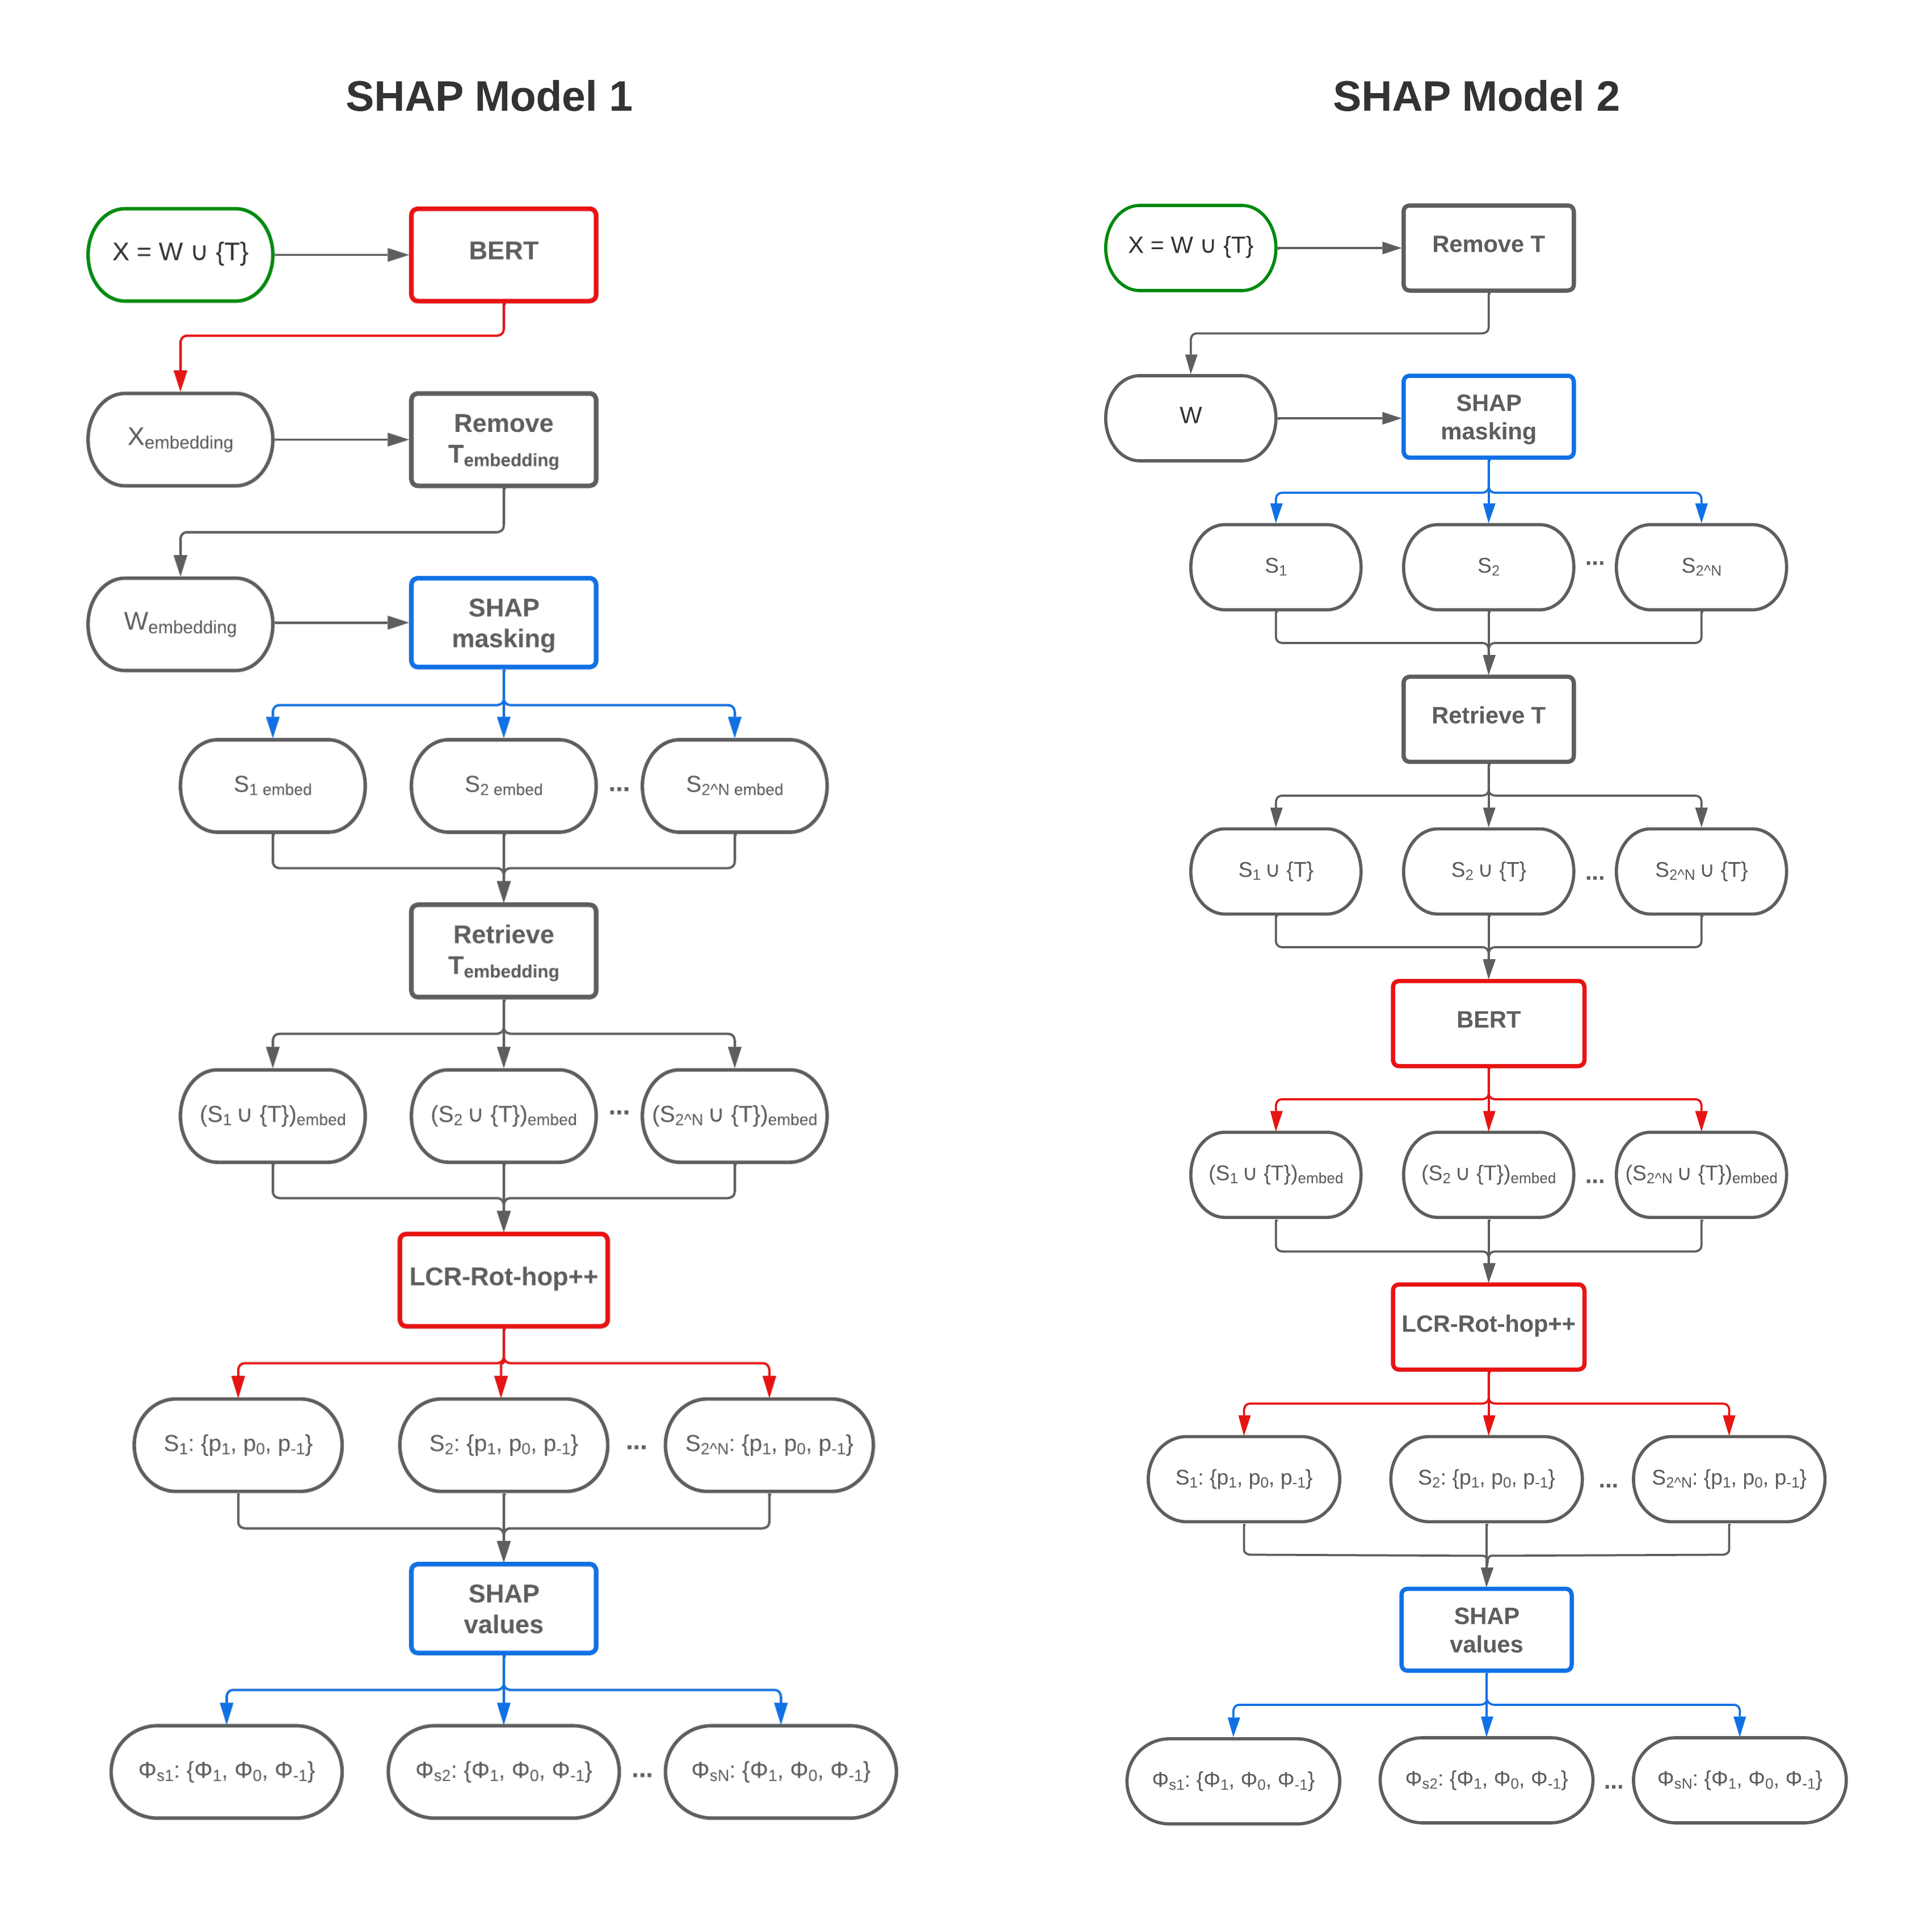
\includegraphics[width=150mm]{figures/SHAP model 1+2.png}
    \caption{SHAP integrated within LCR-Rot-hop++}
    \label{fig:shap_model}
\end{figure}